\chapter{Impose spectra}
%

% - Purpose & Problem description:
%     These first two parts give reader short details about the test case,
%     the physical phenomena involved and specify how the numerical solution will be validated
\section{Description of the problem}
%
%purpose
This example shows how to impose spectra on the boundary of a nested grid in
\tomawac. To do so, two simulations are done. One on a larger domain, which we
will call the oceanic mesh, and another smaller mesh which fits inside the
first mesh. This second mesh will be called the Coastal mesh, and as it is
often the case, it will be more refined than the Oceanic mesh. The larger mesh
will be used to force the smaller mesh. The only requirement to do this, is
that all the points on the open boundary of the smaller mesh need to be present
in the larger mesh. This is illustrated in
\figurename~\ref{fig:impose_spectra_meshes}.

The geometrical parameters of the meshes can be found in
\tablename~\ref{tab:impose_spectra_meshes}.

\begin{table}[H]
\begin{center}
%
\caption{Geometrical parameters for the meshes used in this test case.}
\label{tab:impose_spectra_meshes}
%
\begin{tabular*}{0.7\linewidth}{@{\extracolsep{\fill}}ccc}
\toprule
\toprule
 & \textbf{Oceanic Mesh} & \textbf{Coastal Mesh} \\
\midrule
Number of elements      & 3676 & 4596  \\
Number of nodes         & 1899 & 2460  \\
Maximum edge length (m) & 10.0 & 10.9  \\
Minimum edge length (m) & 4.73 & 0.803 \\
\bottomrule
\bottomrule
\end{tabular*}
%
\end{center}
\end{table}

The energy spectrum will be decomposed in $36$ directions and $32$ frequencies.
The minimal frequency is equal to $0.04$ Hz and the frequential ratio is
$1.055$. The initial water depth is $5$ m. The modelling time step is equal to
$1$ s, and the simulation will run for $100$ time steps (which is enough to
reach a steady state. $3$ subiterations will be used to compute the source
terms.

Since this is a non-regression test, several modelling options could have been
chosen, and the choices made will now be listed for reproducibility. To
generate the waves a uniform wind will blow over the whole domain. Its velocity
is equal to $(20,0)$ m/s. The \texttt{WIND GENERATION} is in accordance with
WAM cycle 3 \citep{Snyder1981}. \texttt{WHITE CAPPING DISSIPATION} is in
accordance with Van des Westhuysen (2007) \citep{Westhuys2007}. \texttt{BOTTOM
  FRICTION DISSIPATION} is in accordance with WAM cycle 4
\citep{Hasselmann1973,Bouws1983}. \texttt{DEPTH-INDUCED BREAKING DISSIPATION}
is in accordance with Thornton et Guza  (1983) \citep{Thornton1983}.
\texttt{NON-LINEAR TRANSFERS BETWEEN FREQUENCIES} follows WAM cycle 4 (DIA
Method) \citep{Hasselmann1985_1}. The \texttt{LINEAR WAVE GROWTH} follows
Cavaleri and Malanotte-Rizzoli (1981) \citep{Cavaleri1981,Tolman1992}.

\begin{figure}[H]
\begin{center}
	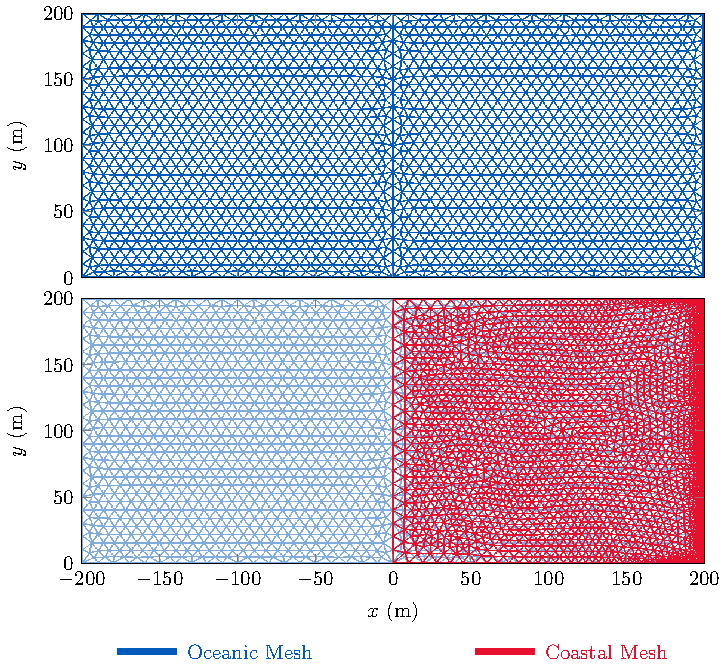
\includegraphics[width=0.8\textwidth]{./Figures/MeshIllustration.pdf}
\end{center}
\caption{Illustration of the meshes of the test case. The mesh in
  {\color{EdfBlue} blue} is the large
  Oceanic mesh, and the mesh in {\color{PantoneRed} red} is the smaller nested
  Coastal mesh.}
\label{fig:impose_spectra_meshes}
\end{figure}
%

% - Numerical parameters:
%     This part is used to specify the numerical parameters used
%     (adaptive time step, mass-lumping when necessary...)
%
%
\section{Numerical parameters}
%
To force the Coastal simulation with the Oceanic results, the spectra of the
points in the Oceanic mesh that are on the open boundary of the Coastal mesh
need to be outputed.This is done most easily using an external text file
containing a list of the coordinates of the points to output. In the steering
file of the Coastal mesh this given using the following keyword:

\lstset{language=TelemacCas,
        basicstyle=\scriptsize\ttfamily}

\begin{lstlisting}[frame=trBL]
/--------------------------------------------------------------------/
/ WRITING SPECTRA
/--------------------------------------------------------------------/
PUNCTUAL RESULTS FILE = './OceanicResults.spe'
FILE WITH COORDINATES OF SPECTRA TO WRITE =
'./SpectraOutputOceanic.dat'
\end{lstlisting}

On the Coastal mesh, these spectra are then imposed on the open boundary. To do
so, the points along the open boundary need to have the boundary condition
\verb+5 4 4 4+. The imposed spectra file, and the coordinates of each spectra
are given using the following keywords:

\lstset{language=TelemacCas,
        basicstyle=\scriptsize\ttfamily}

\begin{lstlisting}[frame=trBL]
/--------------------------------------------------------------------/
/ IMPOSE SPECTRA ON THE OPEN BOUNDARY
/--------------------------------------------------------------------/
IMPOSED SPECTRA FILE = './OceanicResults_dt10.spe'
/IMPOSED SPECTRA FILE FORMAT = 'SERAFIN '
FILE WITH COORDINATES OF SPECTRA TO IMPOSE =
'./SpectraOutputOceanic.dat'
/TIME UNIT OF IMPOSED SPECTRA FILE = 1.
/TIME SHIFT OF IMPOSED SPECTRA FILE = 0.
\end{lstlisting}

%
% - Results:
%     We comment in this part the numerical results against the reference ones,
%     giving understanding keys and making assumptions when necessary.
%
%
\section{Results}

This test case serves mostly to illustrate how to impose spectra from a large
mesh on a smaller nested mesh. Therefore, it will only serve as a
non-regression test. The first check is to find the differences on the
two-dimensional mesh with the reference file, see
\tablename~\ref{tab:impose_spectra_2D}.

%\begin{landscape}
%\begin{small}
%
\begin{table}[H]
\begin{center}
%
%\small
\footnotesize
%
\caption{Summary of the differences with the reference files for the 2D results.
  The last column is the maximum accepted difference.}
\label{tab:impose_spectra_2D}
%
%\input{../table/tab_r2d.tex}
\includetablemaybe{../table/tab_r2d.tex}
%
\end{center}
\end{table}
%
%\end{small}
%\end{landscape}

The spectra on the nodes along the open boundary of the Coastal mesh will also
be checked for non-regression. These spectra are checked with the reference
file, and between the Oceanic and Coastal results. This last check is to ensure
that what is imposed is the same as what is seen in the code.
See \tablename~\ref{tab:impose_spectra_Spe}.

%\begin{landscape}
%
\begin{table}[H]
\begin{center}
%
\small
%
\caption{Summary of the differences with the reference files for the spectra
  results. Note, the name of the variables are only true for the Oceanic
  results. The last column is the maximum accepted difference.}
\label{tab:impose_spectra_Spe}
%
%\input{../table/tab_spe.tex}
\includetablemaybe{../table/tab_spe.tex}
%
\end{center}
\end{table}
%
%\end{landscape}

Nonetheless, even if the spectra along the open boundary of the Coastal mesh is
the same as in the Oceanic mesh, there are differences in the domain (due to
the nature of the boundary conditions). This is illustrated with the last
columns $6$ ans $7$ of \tablename~\ref{tab:impose_spectra_2D}. These
differences are minimal, as can be seen in
\figurename{}s~\ref{fig:impose_spectra_Hm0}-\ref{fig:impose_spectra_WSpread},
where the values along a cross-section taken at $y=100$ m are plotted.

\begin{figure}[H]
\begin{center}
  \includegraphicsmaybe{[width=0.7\textwidth]}{../img/wave_height_hm0.png}
\end{center}
\caption{Cross-section of the wave height $H_{m0}$ along $y=100$ m for the
  Oceanic and Coastal
simulations. Note, only the scalar simulations are compared.}
\label{fig:impose_spectra_Hm0}
\end{figure}

\vfill\mbox{}

\begin{figure}[H]
\begin{center}
  \includegraphicsmaybe{[width=0.7\textwidth]}{../img/mean_period_tmoy.png}
\end{center}
\caption{Cross-section of the wave period $t_{moy}$ along $y=100$ m for the
  Oceanic and Coastal
simulations. Note, only the scalar simulations are compared.}
\label{fig:impose_spectra_Tmoy}
\end{figure}

\begin{figure}[H]
\begin{center}
  \includegraphicsmaybe{[width=0.7\textwidth]}{../img/wave_spread.png}
\end{center}
\caption{Cross-section of the wave spread along $y=100$ m for the Oceanic and
  Coastal simulations.
Note, only the scalar simulations are compared.}
\label{fig:impose_spectra_WSpread}
\end{figure}



